%%%%%%%%%%%%%%%%%%%%%%%%%%%%%%%%%%%%%%%%%%%%%%%%%%%%%%%%%%%%
% Dokument-Einstellungen
\documentclass{SMBV12}

\setcounter{tocdepth}{5} %to make it appears in TOC
\setcounter{secnumdepth}{5} %to make it numbered

%%%%%%%%%%%%%%%%%%%%%%%%%%%%%%%%%%%%%%%%%%%%%%%%%%%%%%%%%%%%
%-----------------------------------------------------------
% Hier beginnt das eigentliche Dokument
\begin{document}

\title{Graph-Based Segmentation}

\author{Phan-Anh Nguyen}

\maketitle

%%%%%%%%%%%%%%%%%%%%%%%%%%%%%%%%%%%%%%%%%%%%%%%%%%%%%%%%%%%%
%-----------------------------------------------------------% Zusammenfassung

\begin{abstract}%
Abstract. This 20-page seminar paper reviews the state-of-the-art graph-based segmentation algorithms.
\end{abstract}

\keywords{Classification, Graph Cut, Segmentation}


%%%%%%%%%%%%%%%%%%%%%%%%%%%%%%%%%%%%%%%%%%%%%%%%%%%%%%%%%%%%
%-----------------------------------------------------------
%
\section{Introduction}

Introduction is written at last.

%%%%%%%%%%%%%%%%%%%%%%%%%%%%%%%%%%%%%%%%%%%%%%%%%%%%%%%%%%%%
%-----------------------------------------------------------
%
\section{Image Features}

%%%%%%%%%%%%%%%%%%%%%%%%%%%%%%%%%%%%%%%%%%%%%%%%%%%%%%%%%%%%
\subsection{Image Feature Overview}
%What are image features? How can we describe/represent them?
Low level image features are essential building blocks for high level image processing tasks such as object detection, image categorization or segmentation etc. In general, image features capture important properties over image regions in various forms that can be used by high level applications. Features often come in two form: point-based features describing salient points in an image and shape-based features containing geometric information such as contours. In this section we present the methods to detect and represent these two kind of features. Specifically, Section $\ref{sec:surf}$ describes a state-of-the-art point-based feature called SURF (Speeded Up Robust Features) \cite{bay2006surf} and Section $\ref{sec:shape_feature}$ shows the methods to extract shape-based features.


%%%%%%%%%%%%%%%%%%%%%%%%%%%%%%%%%%%%%%%%%%%%%%%%%%%%%%%%%%%%
\subsection{SURF Feature}
\label{sec:surf}
Since SURF \cite{bay2006surf} is a point-based feature, we need a method to detect interest points in the input image. The choice of the detector varies depending on the application need. In an image registration application, it is required that the same interest points be detected in two different images of the same scene under different viewing conditions. In this case, the good detector would pick up corner points. In the case of image segmentation, it would be a wise choice to select points on contours to be interest points. In the original SURF paper, Bay et al. suggested using approximate Hessian detector to search in scale-space domain for points having strong derivatives in two orthogonal directions as interest points (often located at corners and strongly textured areas).

Given an interest point in the input image, the SURF descriptor is obtained by extracting distinctive information around its neighbourhood in a form of a feature vector. The SURF descriptor is designed to be invariant to image scaling and rotation while it has to be computed very fast. Scale invariance is achieved by adopting the scale at which the Hessian detector attains maximal response. In order to be invariant to rotation, we first find a reproducible orientation based on information within a circular region around the interest point. We then construct a square region aligned to the selected orientation and extract the SURF descriptor from it.

To find the dominant orientation, the Haar wavelet responses in $x$ and $y$ directions, ($d_x$, $d_y$), are calculated within a circular neighbourhood of radius $6s$ around the interest point and weighted with a Gaussian ($\sigma = 2s$), where $s$ is the scale chosen above. Figure $\ref{fig:haar_wavelet}$ shows the structure of the Haar wavelet filters. The wavelet responses ($d_x, d_y$) are then represented in a vector space and the sum of all vectors within a sliding orientation window of size $\pi/3$ are calculated, see Figure $\ref{fig:orientation_window}$. The dominant orientation is finally assigned to the sum vector having the maximal length.

\begin{figure}[htbp]
    \centering
    \subfigure[]
    {
        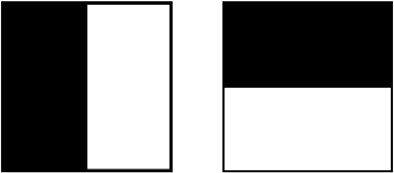
\includegraphics[width=0.15\textwidth]{images/haar_wavelet.png}
        \label{fig:haar_wavelet}
    }
    \subfigure[]
    {
        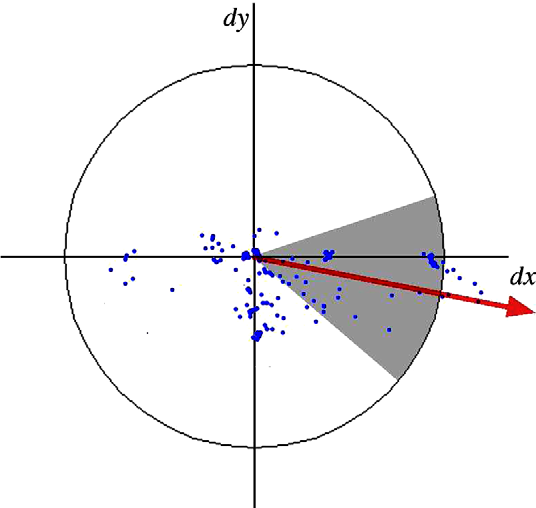
\includegraphics[width=0.25\textwidth]{images/orientation_window.png}
        \label{fig:orientation_window}
    }
    \subfigure[]
    {
        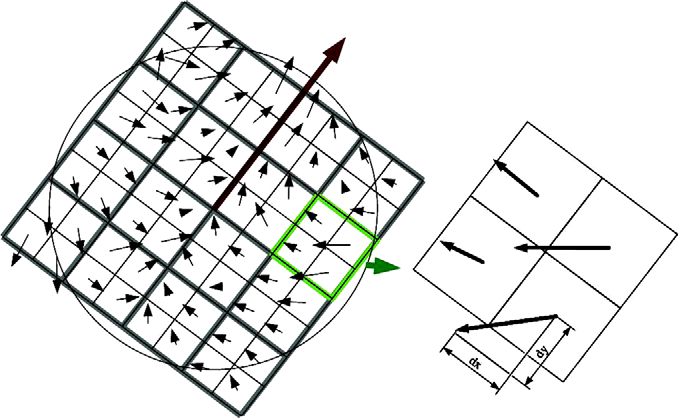
\includegraphics[width=0.5\textwidth]{images/surf.png}
        \label{fig:surf}
    }
    \caption{(a) Haar wavelet filters for the x (left) and y (right) components. The dark parts are weighted -1 and the light parts +1. (b) Orientation assignment: a sliding orientation window of size $\pi/3$ detects the dominant orientation. (c) The SURF descriptor: an oriented quadratic grid with $4 \times 4$ square cells is laid over the interest point (left). For each cell, the wavelet responses are computed from $5 \times 5$ samples (for illustrative
    purposes, only $2 \times 2$ sub-divisions are shown here). In each cell, the 4 elements $\sum d_x$, $\sum \left| d_x \right|$, $\sum d_y$, $\sum \left| d_y \right| $ contribute to the SURF feature vector. } 
    %\label{fig:surf}
\end{figure}

To extract the SURF descriptor, we construct a window of size $20s$ centred at the interest point and oriented in the dominant orientation as illustrated in Figure $\ref{fig:surf}$. The window is then subdivided into a regular $4 \times 4$ grid cells, each being a $5 \times 5$ pixel patch. For each cell, the Gaussian weighted ($\sigma = 3.3s$) Haar wavelet responses are summed up to form a first set of entries in the feature vector. The sum of the absolute values of the responses, $\left| d_x \right| $ and $\left| d_y \right| $ are also extracted to capture information about the polarity of the intensity changes. Therefore, each cell has a 4D descriptor vector for its underlying intensity structure $\left( \sum d_x, \sum d_y, \sum \left| d_x \right| , \sum \left| d_y \right|  \right)$. Concatenating this for all $4 \times 4$ cells results in a descriptor vector of length 64. Finally the descriptor vector is normalized to make it invariant to contrast.

%%%%%%%%%%%%%%%%%%%%%%%%%%%%%%%%%%%%%%%%%%%%%%%%%%%%%%%%%%%%
\subsection{Edges and Contours}
\label{sec:shape_feature}

\subsubsection{Canny Edge Detector}

\subsubsection{gPb Contour Detector}

\cite{maire2008using}
\cite{martin2004learning}

\subsubsection{Measuring Contour Saliency}

\cite{arbelaez2009contours}

\subsubsection{Shape Descriptor}

\cite{gu2009recognition}

%%%%%%%%%%%%%%%%%%%%%%%%%%%%%%%%%%%%%%%%%%%%%%%%%%%%%%%%%%%%
\subsection{Discussion}

pros and cons. Which descriptor is suitable for a particular case.

\section{Supervised versus Unsupervised Segmentation Approaches}



\subsection{Supervised Approaches}

\subsubsection{Region Classification}

\paragraph{Bag of Visual Words}

\paragraph{Support Vector Machine}

\paragraph{Structured SVM learning framework}

\cite{tsochantaridis2006large}

\subsubsection{Statistical Shape Model}

\cite{leventon2000statistical}

\subsection{Unsupervised Approaches}



\section{Graph Construction}

Intuitive connection between graphs and images.

\subsection{Region Graph}

\cite{arbelaez2009contours}

Vertex weight: point, shape features quantized by K-mean.
Edge weight: contour strength quantized by L-bin histogram and trained by the structured SVM learning framework.

Graph of small over-segmented regions. What is the advantage of this representation compared to branch and bound scheme. MWCS and PCST

\subsection{Contour Graph}

Circulation and Circle Embedding

\subsection{Markov Random Field}

\section{Graph Cut Algorithms}

comparison of cut algorithms, could them be used interchangeably in different situations.

\subsection{Prize-Collecting Steiner Tree}

\cite{ljubic2006algorithmic}

\subsubsection{Branch-and-Cut Algorithm}

\subsection{Hermitian Eigenvalue Problem}

\subsubsection{Normalized Cut}

\cite{shi2000normalized}

\subsubsection{Contour Cut}

\cite{zhu2007untangling}
\cite{KenGalShi2011}

\subsection{Graph-Cut}

\subsubsection{Min-Cut}

\subsubsection{Alpha-Expansion and Fusion Move}

\section{Applications}

System pipeline, result: accuracy, efficiency, benefits.

\subsection{Efficient Region Search for Object Detection}

\cite{VijayGrauman2011}

\subsection{Salient Contour Detection}

\cite{KenGalShi2011}

\subsection{Multi-Shape Graph-Cut for Lung Segmentation}

\cite{nakagomimulti}

\section{Conclusion}

lack of information: SURF at Canny points: what scale?
some criticisms e.g. time consuming, dataset used. Recommendation: what to use, why?

%%%%%%%%%%%%%%%%%%%%%%%%%%%%%%%%%%%%%%%%%%%%%%%%%%%%%%%%%%%%
%-----------------------------------------------------------
%
\def\refname{Literature}
%\begin{thebibliography}{AA}

\bibliographystyle{alpha}
\bibliography{bibliography}

%\end{thebibliography}

\newpage
\noindent
\begin{picture}(160,242)
\put(0,0){\framebox(160,242){}}
\end{picture}

\end{document}
